\chapter{相关技术介绍}
\section{Spark平台介绍}
Apache Spark是为了快速计算而设计出来的集群计算计数。它基于Hadoop MapReduce技术,并且扩展了Hadoop MapReduce模型来有效地进行更多类型的计算,包括想交互式查询以及流处理。Spark最主要的特性是内存集群计算技术,将数据保持在内存而不序列化到硬盘上大大提高了计算速度。

Spark最早是由UC Berkeley的Matei Zaharia在2009年作为Hadoop的一个子项目进行开发的。它在2010年基于BSD整数开源并在2013年捐献给了Apache Software foundation(ASF)。从2014年的二月起,Spark已经成为了ASF中的顶级项目之一。Apache Spark官网将Spark定义为大规模数据处理的一个快速、通用的引擎。

Spark有如下主要特性
\begin{itemize}
    \item \textbf{速度}。如果在内存中,Spark能比Hadoop MapReduce快100倍以上,如果在硬盘上,则能快10被以上。
    \item \textbf{便于使用}。Spark支持Java/Scala/Python/R四种语言的API,提供了超过80多种高度抽象的操作来使得编写并行App更加容易。并且提供了Scala,Python和R的交互式Shell。
    \item \textbf{通用性}。Spark联合了SQL、streaming和complex analytics。Spark由SQL and Dataframes, MLLib for machine learning, GraphX和Spark Streaming驱动。我们可以在同一个App中无缝地联合使用这么多库。
    \item \textbf{随处运行}。Spark可以运行在Hadoop、Mesos、独立模式上,还可以在云上运行。Spark可以访问包括HDFS、Cassandra、HBase和S3等在内的多种数据源。我们可以在独立集群模式下或者EC2或者Hadoop YARN或者Apache Mesos下运行Spark。访问位于HDFS、Cassandra、HBase、Hive、Tachyon和任何Hadoop数据源。
\end{itemize}

Spark有如下主要组成
\begin{figure}[ht]
\centering
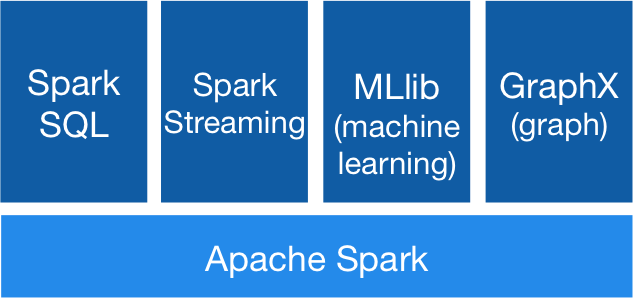
\includegraphics[width=10cm]{spark-stack}
\caption{Spark Stack}
\end{figure}
\begin{itemize}
    \item \textbf{Spark SQL}。Spark SQL使得你可以通过Java、Python、R、Scala语言在Spark程序中使用SQL或者熟悉的DataFrame API来查询结构化数据。并且DataFrames和SQL提供了一种通用的方式来访问多种不同的数据源,包括Hive, Avro, Parquet, ORC, JSON和JDBC。我们甚至可以使用对数据使用join操作。Spark SQL完全兼容Hive操作,我们可以对于已有的数据运行未经修改的Hive查询。通过JDBC和ODBC,我们可以使用标准的连接方式。
    \item \textbf{Spark Streaming}。Spark Streaming提供了Apache Spark语言级整合的API来进行流处理,我们可以像编写批处理任务的代码一样来编写流任务。支持java、Scala、Python。容错性较高,开箱支持从lost work和operator state中恢复。Spark整合性,可以把流处理和批处理以及交互式请求结合起来。
    \item \textbf{Spark MLlib}。方便使用,MLlib可以和Python中的Numpy库进行交互,使用使用任何Hadoop数据源(HDFS, HBase or local files),使得MLlib很容易插入Hadoop workflow中。性能上,高质量算法,比MapReduce快100倍。方便部署,我们可以在Hadoop 2集群上不预装任何东西的情况下运行Spark和MLlib。
    \item \textbf{GraphX}。灵活性,可以在collections和graphs之间无缝整合,GraphX在单个系统中统一了ETL,解释分析,迭代图计算。我们我们把同一份数据视为graphs或者collections,transform或者join graphs。性能上,与其他专门的图处理系统相比是最快的。算法上,拥有很多图算法的实现,包括PageRand, Connected components, label propagations, SVD++, Strongly connected components, Triangle count等。
\end{itemize}

\subsection{Spark部署情况}
Spark中部署情况如图。
\begin{figure}[ht]
\centering
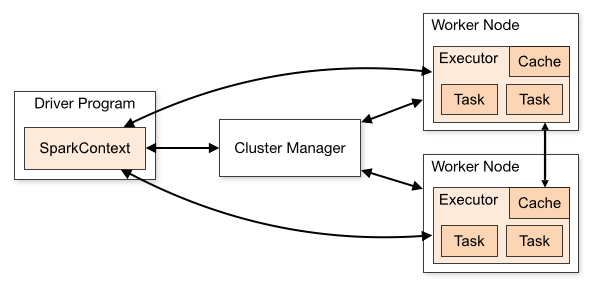
\includegraphics[width=10cm]{cluster-overview}
\caption{cluster overview}
\end{figure}
我们把程序提交到Spark Driver上,由Driver来进行任务调度,实际的计算任务几乎都泡在Spark Nodes上。由于任务调度的关系,Driver和Work Nodes最好能够在同一个局域网下,不然因为网络延迟以及带宽的缘故,花在网络等待的时间可能较长。
\subsection{Spark基本编程模型}
Spark中最基本的数据类型是RDD( Resilient Distributed Dataset)。它可以通过读取Hadoop InputFormat或者通过其他RDD Transform得到。在Spark中由两种最基本的操作transform和action,可以认为是MapReduce的扩展。

% todo 重新transformaton和action表格
%\begin{longtable}{ccc}
%% 首页表头
%\caption[RDD Transformations]{RDD Transformation} \label{tab:rddtrans} \\
%\toprule[1.5pt]
%Transformation  & Meaning\\
%\midrule[1pt]
%\endfirsthead
%% 续页表头
%\caption[]{RDD Tranfromation(Continued)} \\
%\toprule[1.5pt]
%Tranformation & Meaning\\
%\midrule[1pt]
%\endhead
%% 首页表尾
%\hline
%\multicolumn{3}{r}{\small To be continued}
%\endfoot
%% 续页表尾
%\bottomrule[1.5pt]
%\endlastfoot
%map(func)	& Return a new distributed dataset formed by passing each element of the source through a function func.\\
%filter(func)	& Return a new dataset formed by selecting those elements of the source on which func returns true. \\
%flatMap(func)	& Similar to map, but each input item can be mapped to 0 or more output items (so func should return a Seq rather than a single item). \\
%mapPartitions(func)	& Similar to map, but runs separately on each partition (block) of the RDD, so func must be of type Iterator<T> => Iterator<U> when running on an RDD of type T. \\
%mapPartitionsWithIndex(func) &	Similar to mapPartitions, but also provides func with an integer value representing the index of the partition, so func must be of type (Int, Iterator<T>) => Iterator<U> when running on an RDD of type T. \\
%sample(withReplacement, fraction, seed) &	Sample a fraction fraction of the data, with or without replacement, using a given random number generator seed. \\
%union(otherDataset)	& Return a new dataset that contains the union of the elements in the source dataset and the argument. \\
%intersection(otherDataset) &	Return a new RDD that contains the intersection of elements in the source dataset and the argument.\\
%distinct([numTasks]))	& Return a new dataset that contains the distinct elements of the source dataset.\\
%groupByKey([numTasks])	& When called on a dataset of (K, V) pairs, returns a dataset of (K, Iterable<V>) pairs. 
%Note: If you are grouping in order to perform an aggregation (such as a sum or average) over each key, using reduceByKey or aggregateByKey will yield much better performance. 
%Note: By default, the level of parallelism in the output depends on the number of partitions of the parent RDD. You can pass an optional numTasks argument to set a different number of tasks. \\
%reduceByKey(func, [numTasks]) & 	When called on a dataset of (K, V) pairs, returns a dataset of (K, V) pairs where the values for each key are aggregated using the given reduce function func, which must be of type (V,V) => V. Like in groupByKey, the number of reduce tasks is configurable through an optional second argument. \\
%aggregateByKey(zeroValue)(seqOp, combOp, [numTasks])	& When called on a dataset of (K, V) pairs, returns a dataset of (K, U) pairs where the values for each key are aggregated using the given combine functions and a neutral "zero" value. Allows an aggregated value type that is different than the input value type, while avoiding unnecessary allocations. Like in groupByKey, the number of reduce tasks is configurable through an optional second argument. \\
%sortByKey([ascending], [numTasks])	 & When called on a dataset of (K, V) pairs where K implements Ordered, returns a dataset of (K, V) pairs sorted by keys in ascending or descending order, as specified in the boolean ascending argument. \\
%join(otherDataset, [numTasks]) &	When called on datasets of type (K, V) and (K, W), returns a dataset of (K, (V, W)) pairs with all pairs of elements for each key. Outer joins are supported through leftOuterJoin, rightOuterJoin, and fullOuterJoin. \\
%cogroup(otherDataset, [numTasks])	& When called on datasets of type (K, V) and (K, W), returns a dataset of (K, (Iterable<V>, Iterable<W>)) tuples. This operation is also called groupWith.\\
%cartesian(otherDataset)	 & When called on datasets of types T and U, returns a dataset of (T, U) pairs (all pairs of elements). \\
%pipe(command, [envVars])	& Pipe each partition of the RDD through a shell command, e.g. a Perl or bash script. RDD elements are written to the process's stdin and lines output to its stdout are returned as an RDD of strings. \\
%coalesce(numPartitions)	& Decrease the number of partitions in the RDD to numPartitions. Useful for running operations more efficiently after filtering down a large dataset. \\
%repartition(numPartitions) &	Reshuffle the data in the RDD randomly to create either more or fewer partitions and balance it across them. This always shuffles all data over the network. \\
%repartitionAndSortWithinPartitions(partitioner) & 	Repartition the RDD according to the given partitioner and, within each resulting partition, sort records by their keys. This is more efficient than calling repartition and then sorting within each partition because it can push the sorting down into the shuffle machinery \\
%\end{longtable}


\section{推荐系统介绍}
推荐系统在现在的场景中越来越重要,由于信息的爆炸式增加,互联网上的商品数量也在不断的增加,但是用户能够浏览的信息和商品都是有限的,如何让用户浏览他们需要的东西成为商品/服务提供者所面临的一个问题,引起了人们对于推荐系统的研究。推荐系统最早是由美国明尼苏达大学的小组进行研究的,目前针对推荐系统的研究较为广泛,推荐系统的应用也较为普遍。目前的推荐系统主要可以分为个性化推荐系统与非个性化推荐系统。个性化会根据针对不同用户推荐不同的数据,而非个性化推荐系统考虑的因素没有用户。除了基于用户评分的推荐算法,推荐系统还有很多变种,比如基于用户显式评分的推荐系统,基于用户隐式评分的推荐系统,基于信任关系的推荐系统。在推荐系统中也很很多值得研究的问题,比如冷启动问题,如何防止恶意用户攻击推荐系统等。
\subsection{算法总览}
%todo 编写顺序算法
在目前的非个性化推荐系统中,主要的实现方法是对每个item用户可以进行点击upvote,upvote比较靠前的就可以排在比较靠前的位置,对于需要考虑时间因素的新闻推荐,会综合考虑upvote数和已经发布的时间,比如在Hacker New网站中,使用的推荐算法是这个链接部分的https://medium.com/hacking-and-gonzo/how-hacker-news-ranking-algorithm-works-1d9b0cf2c08d。比如在知名的reddit网站,推荐算法由如下的数学表示
$$    t_s = A - B$$
$$x = U - D$$
$$ y = 1 if x > 0$$
$$z = |x| if |x| \geq 1$$
\begin{equation}
f(t_s, y, z) = \log_{10}z + \frac{yt_s}{45000}    
\end{equation}

对于评论的推荐算法如下
\begin{equation}
    \frac{\hat{p}+\frac{z^2}{2n}\pm z\sqrt{\frac{\hat{p}(1-\hat{p})}{n}+\frac{z^2}{4n^2}}}{1+\frac{z^2}{n}}
\end{equation}
这两部分是比较成功的推荐系统。

对于个性化推荐算法推荐算法,主要有我们如下介绍的基于内容过滤和协同过滤两大类,我们将在接下来的章节详细介绍这一部分。

\subsection{基于内容过滤的推荐算法}
基于内容过滤的推荐算法,根据一个用户消费的商品与其他的商品的相似性来进行推荐。而商品之间的相似性是通过用户评分之外的信息来计算,适合于在能够获取商品较多的信息下使用。使用基于内容过滤算法的推荐系统,不会遇到冷启动问题。关键在于对描述商品的信息的选取,通常情况下我们会使用tags作为商品的信息描述,tags的添加可以通过人工录入或者机器学习的方式的录入。每个tags视为一个维度,这样我们可以将一个商品表示成依赖tags的一个向量,通过计算两个向量之间的相似性,我们可以得出商品之间的相关性。我们需要注意的几个问题有,商品之间的tags可能是同义tags,所以需要注意tags的选取。

基于内容过滤的推荐算法,避免了冷启动问题,不会有商品因为刚加入系统时候缺少用户评分而无法推荐给用户。并且这样相似性计算可以可以解释。

\subsection{基于邻域的推荐算法}
    \begin{equation}
       similarity(\vec{A}, \vec{B}) = cosine(\vec{A}, \vec{B}) = \frac{\vec{A} \cdot \vec{B}}{\lVert\vec{A}\rVert\ast\lVert\vec{B}\rVert}
    \end{equation}

\subsubsection{相似关系}
基于领域的

\subsubsection{用户与用户之间的相似关系}
每个用户和其他用户之间的相似关系可以通过该用户给消费过的物品评分来计算。我们可以认为每个物品都是一个维度,每个用户都是在高维空间的一个向量。我们可以通过计算两个用户共同评分过的的物品的之间的夹角。通过夹角的大小我们来评估用户之间的相似性。当夹角超过90度的时候,我们认为用户之间存在负相关性。这种负相关性不需要出现在我们的用户的邻居中,需要剔除掉。
\subsubsection{物品与物品之间的相似关系}
介绍计算相似性的时候,注意讲一下在相似性计算的时候,存在一个问题,就是如果一个item-item pair只有一个用户评分的话,那么他们之间的相似性必然为1,我们在计算相似性的时候,要去掉这种情况。
\subsection{ALS算法}
ALS算法是讲一个矩阵分解成两个维度较小的矩阵。